% # -*- coding:utf-8 -*-
\documentclass[10pt,aspectratio=169,mathserif]{beamer}		

\usepackage{zju}
\usepackage{ctex}
\usepackage{amsmath,amsfonts,amssymb,bm}
\usepackage{color}
\usepackage{graphicx,hyperref,url}
\usepackage{metalogo}
\usepackage{mathptmx}
\usepackage{times}
\usepackage{textcomp}
\usepackage{subcaption}

\newcommand{\code}[1]{\texttt{\small {\detokenize{#1}}}}

\usepackage[OT1]{fontenc} 
\usepackage{fontspec}
\setmonofont{Fira Code}

\usefonttheme{serif}

\beamertemplateballitem

\title{标题}

\subtitle{副标题}			

\author{王行楷}
  
\institute{浙江大学}

\date{\today{}}
  
\begin{document}

\begin{frame}
	\titlepage
\end{frame}

% \section{Outline}
\begin{frame}
	\frametitle{提纲}
	\tableofcontents
\end{frame}

\section{研究动机}
\begin{frame}{动机}
	\textbf{内容}
	\\
	\code{code i think}
\end{frame}

\section{背景}
\begin{frame}{已有工作}
	\begin{figure}
		\centering
		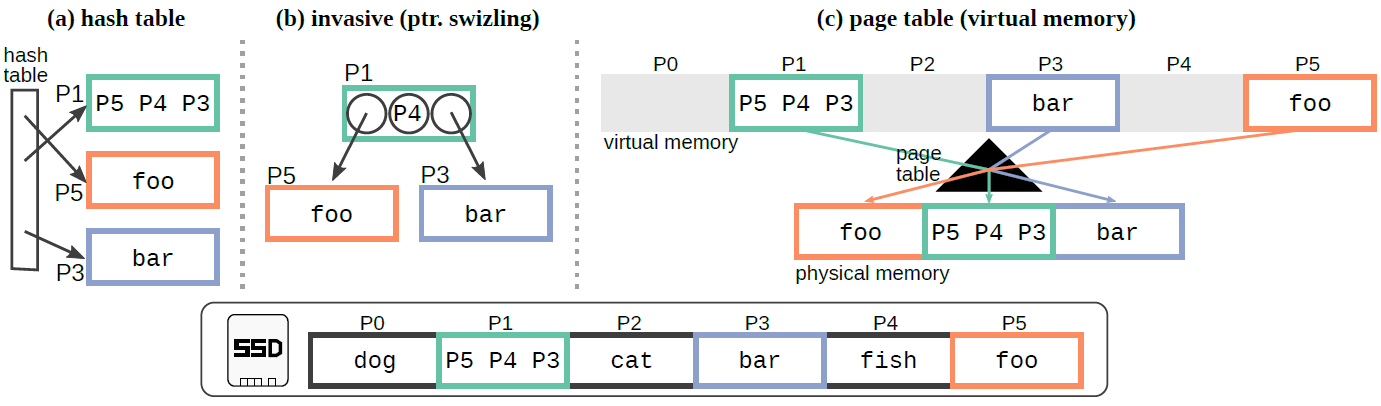
\includegraphics[width=13cm]{./images/existing.png}
		\caption{标题}
	\end{figure}
\end{frame}

\begin{frame}{标题}
	\begin{figure}
		\centering
		\begin{subfigure}{0.65\linewidth}
			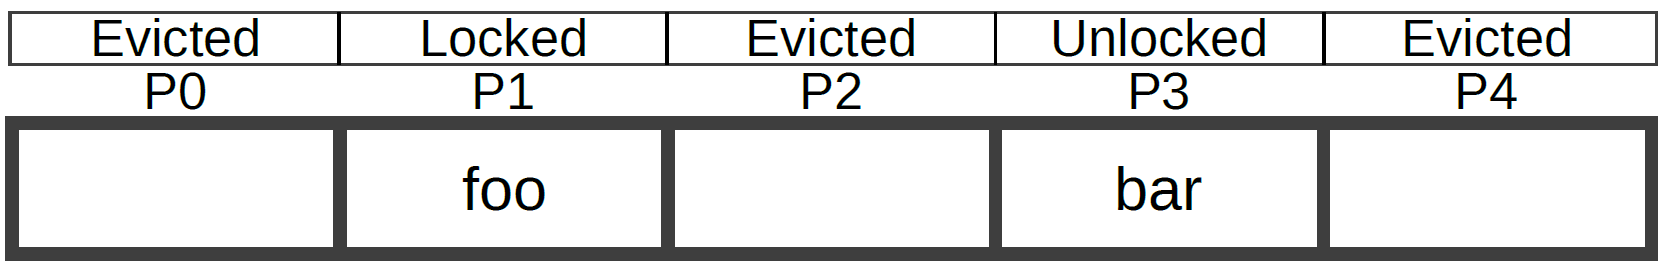
\includegraphics[width=\linewidth]{./images/states.png}
			\caption{子标题}
		\end{subfigure}
		\begin{subfigure}{0.28\linewidth}
			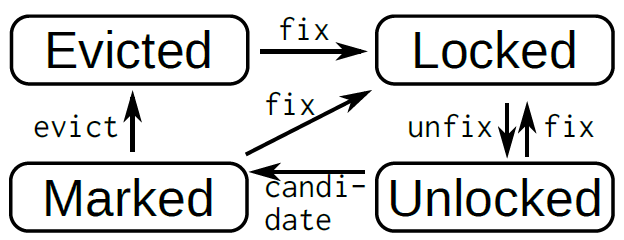
\includegraphics[width=\linewidth]{./images/transfer.png}
			\caption{子标题}
		\end{subfigure}
		\caption{标题}
	\end{figure}
\end{frame}

% \section{参考文献}
% \begin{frame}{参考文献}
% 	\begin{thebibliography}{99}
% 		\bibitem{zhao1} Yi~Zhao, {\sl An introduction to X}, Sep.~15, 2015
% 		\bibitem{qian2} Er~Qian, San~Sun,
% 		Phys.\ Lett.\ A {\bf xx}, 2xx (20xx)
% 		\bibitem{li4} Si~Li, Phys.\ Rev.\ C {\bf xx}, 5xx (20xx)

% 	\end{thebibliography}
% \end{frame}

\end{document}